\documentclass[aspectratio=169]{beamer}
\useoutertheme[progressbar=frametitle]{metropolis}
\useinnertheme{metropolis}
\definecolor{nabgray}{rgb}{0.6,0.59,0.61}
\usecolortheme[named=nabgray]{structure}

\usepackage{tikz}
\usepackage[utf8]{inputenc}
\usepackage[spanish]{babel}

\usepackage{smartdiagram}
\usepackage{qtree}
\usepackage{verbatim}
\usepackage{svg}
\usepackage{graphicx}
\usepackage{color}

\definecolor{lightgray}{rgb}{0.95, 0.95, 0.95}
\definecolor{darkgray}{rgb}{0.4, 0.4, 0.4}
%\definecolor{purple}{rgb}{0.65, 0.12, 0.82}
\definecolor{editorGray}{rgb}{0.95, 0.95, 0.95}
\definecolor{editorOcher}{rgb}{1, 0.5, 0} % #FF7F00 -> rgb(239, 169, 0)
\definecolor{editorGreen}{rgb}{0, 0.5, 0} % #007C00 -> rgb(0, 124, 0)
\definecolor{orange}{rgb}{1,0.45,0.13}		
\definecolor{olive}{rgb}{0.17,0.59,0.20}
\definecolor{brown}{rgb}{0.69,0.31,0.31}
\definecolor{purple}{rgb}{0.38,0.18,0.81}
\definecolor{lightblue}{rgb}{0.1,0.57,0.7}
\definecolor{lightred}{rgb}{1,0.4,0.5}
\definecolor{ocherCode}{rgb}{1, 0.5, 0} % #FF7F00 -> rgb(239, 169, 0)
\definecolor{blueCode}{rgb}{0, 0, 0.93} % #0000EE -> rgb(0, 0, 238)
\definecolor{greenCode}{rgb}{0, 0.6, 0} % #009900 -> rgb(0, 153, 0) 


\usepackage{upquote}
\usepackage{listings}
\lstdefinelanguage{JavaScript}{
	morekeywords=[1]{break, continue, delete, else, for, function, if, in,
		new, return, this, typeof, var, void, while, with},
	% Literals, primitive types, and reference types.
	morekeywords=[2]{false, null, true, boolean, number, undefined,
		Array, Boolean, Date, Math, Number, String, Object},
	% Built-ins.
	morekeywords=[3]{eval, parseInt, parseFloat, escape, unescape},
    % Basic design
    backgroundcolor=\color{lightgray},
    basicstyle={\small\ttfamily},   
    frame=l,
    keywordstyle=\footnotesize\color{blue},
    escapeinside={<@}{@>},
    breaklines=true,
    % Line numbers
    xleftmargin={0.75cm},
    numbers=left,
    stepnumber=1,
    firstnumber=1,
    numberfirstline=true
    % Code design
    identifierstyle=\color{black},
    keywordstyle=\color{ocherCode}\bfseries,
    ndkeywordstyle=\color{greenCode}\bfseries,
    stringstyle=\color{ocherCode}\ttfamily,
    commentstyle=\color{darkgray}\ttfamily,
    tabsize=2,
    showtabs=true,
    showspaces=false,
    showstringspaces=false,
    extendedchars=true,
    breaklines=true
}[keywords, comments, strings]

\colorlet{punct}{red!60!black}
\definecolor{background}{HTML}{EEEEEE}
\definecolor{delim}{RGB}{20,105,176}
\colorlet{numb}{magenta!60!black}

\lstdefinelanguage{json}{
	basicstyle=\normalfont\ttfamily,
	numbers=left,
	numberstyle=\scriptsize,
	stepnumber=1,
	numbersep=8pt,
	showstringspaces=false,
	breaklines=true,
	frame=lines,
	literate=
	*{0}{{{\color{numb}0}}}{1}
	{1}{{{\color{numb}1}}}{1}
	{2}{{{\color{numb}2}}}{1}
	{3}{{{\color{numb}3}}}{1}
	{4}{{{\color{numb}4}}}{1}
	{5}{{{\color{numb}5}}}{1}
	{6}{{{\color{numb}6}}}{1}
	{7}{{{\color{numb}7}}}{1}
	{8}{{{\color{numb}8}}}{1}
	{9}{{{\color{numb}9}}}{1}
	{:}{{{\color{punct}{:}}}}{1}
	{,}{{{\color{punct}{,}}}}{1}
	{\{}{{{\color{delim}{\{}}}}{1}
	{\}}{{{\color{delim}{\}}}}}{1}
	{[}{{{\color{delim}{[}}}}{1}
	{]}{{{\color{delim}{]}}}}{1},
}
\usebackgroundtemplate%
{%
	
\includegraphics[width=\paperwidth]{Images/Contenido}%
}


\title{Mejorando la calidad de código con ECMA 6 y TypeScript}
\author{Víctor Orozco}
\institute{@tuxtor}
\date{\today}

\begin{document}
    
    
{
    \usebackgroundtemplate{
\includegraphics[width=\paperwidth]{Images/portada}}
    \setbeamercolor{frametitle}{fg=red}
    \usebeamercolor[fg]{normal text}
    \frame{\titlepage}
}

\begin{frame}{JavaScript}
\begin{figure}
	\centering
	
\includegraphics[width=0.9\linewidth]{Images/jsframework}
\end{figure}
\end{frame}


\begin{frame}{Clientes JavaScript}
1995-2012: JavaScript es malo! - Developer X con conocimientos de otro lenguaje que no sea JS.
\begin{itemize}
	\item Orientado a hacks
	\item Imperativo (manipulación DOM)
\end{itemize}

\begin{itemize}
	\item 2009: Node.js
	\item 2009: CoffeeScript
	\item 2011: Dart
	\item \textbf{2012: TypeScript}
	\item \textbf{2015: ECMA 6}
\end{itemize}

\end{frame}

\begin{frame}{Clientes JavaScript/HTML5}
\begin{itemize}
	\item Rich clients = HTML+JS+CSS3
	\item MVVM +- MVC del lado del cliente
	\item JSON/XML
	\item Rest - Request-response
	\item Websockets - Full duplex
\end{itemize}
\end{frame}


\begin{frame}{Arquitectura 2015}
\begin{figure}
	\centering
	
\includegraphics[width=0.8\linewidth]{Images/embernode.png}
\end{figure}
\end{frame}

\begin{frame}{Arquitectura 2017}
\begin{figure}
\centering

\includegraphics[width=0.8\linewidth]{Images/knockoutnet.png}
\end{figure}
\end{frame}

\begin{frame}{Arquitectura 2019}
\begin{figure}
\centering

\includegraphics[width=0.8\linewidth]{Images/anguaree.png}
\end{figure}
\end{frame}

\begin{frame}{Clientes JavaScript}
	\begin{itemize}
		\item AJAX (Microsoft)
		\item jQuery, YUI, Dojo
		\pause \item GWT, Icefaces/Primefaces, Vaadin
		\pause \item HTML5, CSS3, WebSockets, WebRTC, HTML Components
		\pause \item AngularJS, Knockout.js, Ember.js
		\pause \item 2013: React, 2014: Vue (DIY/Biblioteca)
		\pause \item 2015: Oracle JET, 2016: Angular, 2019: Nuxt.js (Framework)
	\end{itemize}
	Clave MVVM
\end{frame}


\begin{frame}{Clientes JavaScript}
\begin{itemize}
	\item AJAX (Microsoft)
	\item jQuery, YUI, Dojo
	\pause \item GWT, Icefaces/Primefaces, Vaadin
	\pause \item HTML5, CSS3, WebSockets, WebRTC, HTML Components
	\pause \item AngularJS, Knockout.js, Ember.js
	\pause \item 2013: React, 2014: Vue (DIY/Biblioteca)
	\pause \item 2015: Oracle JET, 2016: Angular, 2019: Nuxt.js (Framework)
\end{itemize}
Clave MVVM
\end{frame}


\begin{frame}{Clientes JavaScript - Resumen}
\begin{itemize}
	\item \textbf{JS, TS}, Dart, CoffeeScript (lenguajes)
	\item \textbf{Angular}, Nuxt.js (frameworks)
	\item \textbf{Webpack}, Parcel, Brocoli (SCM)
	\item \textbf{npm}, yarn (Dependencias)
\end{itemize}
\end{frame}

{
    \usebackgroundtemplate{
\includegraphics[width=\paperwidth]{Images/separador}}
    \setbeamercolor{normal text}{fg=white}
    \setbeamercolor{frametitle}{fg=red}
    \usebeamercolor[fg]{normal text}
    \section{TS}
}


\begin{frame}{TypeScript}
\begin{itemize}
	\item Microsoft
	\item Transpila TS -> JS
	\item Idea general: JS + Tipos + ES.Next
	\item Todo código JS es código TS valido
	\item El código JS es difícil de escalar a menos que sean genios
\end{itemize}
\end{frame}

\begin{frame}{TypeScript vs JavaScript}
\begin{itemize}
	\item debug
	\item Autocompetion
	\item Refactoring
	\item Navegación en los IDEs
	\item Linting
\end{itemize}
\end{frame}

\begin{frame}{TypeScript transpiler}
\begin{itemize}
	\item Resultado final es JS idiomatico
	\item Por defecto siempre produce salida
	\item Superset
	\item Tipado estático
\end{itemize}
\end{frame}

\begin{frame}{TS vs JS}
    \begin{figure}
        \centering
        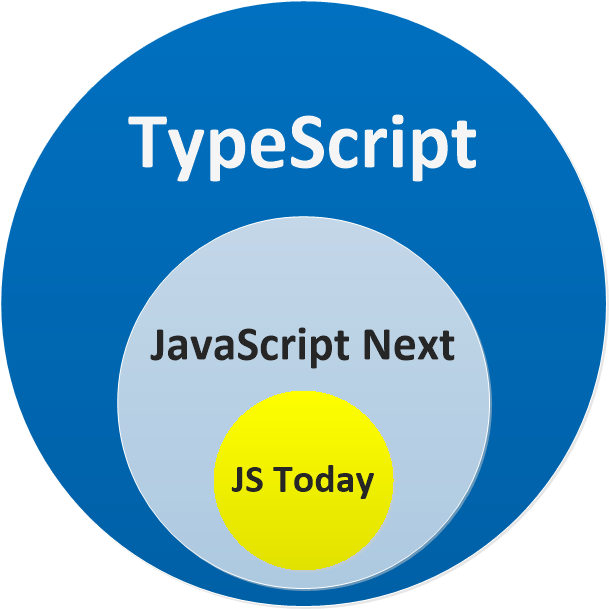
\includegraphics[width=0.5\linewidth]{Images/venn.png}
        \label{fig:requestresponse}
    \end{figure}
    TS es un linter para JS con información de tipos
\end{frame}




\begin{frame}{JS en CLI}
\begin{figure}
	\centering
	
\includegraphics[width=0.8\linewidth]{Images/npmyarn}
\end{figure}
\end{frame}

\begin{frame}[fragile]{TypeScript instalación}
\begin{itemize}
	\item Node.js
	\item Gestor de paquetes
	\item Editor o IDE (VSCode/IntelliJ IDEA)
\end{itemize}

\begin{lstlisting}[language=bash]
npm install -g typescript
npm view typescript version
\end{lstlisting}
Luego
\begin{lstlisting}[language=bash]
tsc -v
\end{lstlisting}
\end{frame}

\begin{frame}[fragile]{TypeScript}

\smartdiagram[sequence diagram]{foo.ts,TS Compiler,foo.js}

\begin{enumerate}
	\item tsc
	\item Webpack
	\item ng-cli
\end{enumerate}
\end{frame}

\begin{frame}[fragile]{TypeScript - Ejercicio 1}

\begin{lstlisting}[language=bash]
tsc ex1.ts
\end{lstlisting}

\begin{lstlisting}[language=JavaScript]
var a = 123
a.trim()
\end{lstlisting}

\end{frame}

\begin{frame}[fragile]{TypeScript - Ejercicio 1}

\begin{lstlisting}[language=bash]
tsc ex1.ts --watch
\end{lstlisting}

\begin{lstlisting}[language=JavaScript]
var a : string = 123
a.trim()
\end{lstlisting}

\end{frame}

\begin{frame}{TypeScript}
\begin{columns}
	\begin{column}{0.5\textwidth}
		\begin{itemize}
			\item Type annotations
			\item Type inference
			\item Compile time type checking
			\item Optional and default params
			\item Classes
			\item Interfaces
			\item Structural typing
			\item Arrow function expression
		\end{itemize}
	\end{column}
	\begin{column}{0.5\textwidth}  %%<--- here
		\begin{itemize}
			\item Enums
			\item Generics
			\item Modules
			\item Tuple types
			\item Union types and type guards
		\end{itemize}
	\end{column}
\end{columns}
\end{frame}

\begin{frame}{TypeScript - Típos}
		\begin{itemize}
			\item Object - any
			\item void - void
			\item boolean - boolean
			\item integer, double . . . - number
			\item String, char - string
			\item Type[] - type[]
		\end{itemize}
\end{frame}


{
    \usebackgroundtemplate{
\includegraphics[width=\paperwidth]{Images/separador}}
    \setbeamercolor{normal text}{fg=white}
    \setbeamercolor{frametitle}{fg=red}
    \usebeamercolor[fg]{normal text}
    \section{NPM}
}


\begin{frame}{NPM}
    \begin{itemize}
        \item Package manager
        \item Task runner (invoker)
        \item Fuerte por la comunidad Node.js
        \item package.json
    \end{itemize}
\end{frame}


\begin{frame}[fragile]{NPM}
    
    \begin{lstlisting}[language=bash]
    mkdir ex2
    cd ex2
    npm init
    \end{lstlisting}
    
    Package.json
    
\end{frame}

\begin{frame}[fragile]{NPM - Package.json}
\begin{lstlisting}[language=JSON]
{
    "name": "ex2",
    "version": "1.0.0",
    "description": "Foo package",
    "main": "index.js",
    "scripts": {
        "test": "echo \"Error: no test specified\" && exit 1"
    },
    "author": "",
    "license": "ISC"
}
\end{lstlisting}

\end{frame}


\begin{frame}[fragile]{NPM - Paquetes}
    https://npmjs.org
\begin{lstlisting}[language=bash]
npm install cowsay
ls -l node_modules
\end{lstlisting}
\end{frame}

\begin{frame}[fragile]{TypeScript - Ejercicio 3}
    
cowsay.ts
\begin{lstlisting}[language=JavaScript]
var cowsay = require("cowsay");

console.log(cowsay.say({
    text : "I'm a moooodule",
    e : "oO",
    T : "U "
}));
\end{lstlisting}

\begin{lstlisting}[language=bash]
node cowsay.js
\end{lstlisting}
    
\end{frame}

\begin{frame}[fragile]{NPM - Resumen}
    \begin{itemize}
        \item npm install
        \item npm install -g
        \item npm install --save
        \item require();
        \item npm uninstall
    \end{itemize}
\end{frame}


{
    \usebackgroundtemplate{
\includegraphics[width=\paperwidth]{Images/separador}}
    \setbeamercolor{normal text}{fg=white}
    \setbeamercolor{frametitle}{fg=red}
    \usebeamercolor[fg]{normal text}
    \section{ECMAScript 6 + TS}
}

\begin{frame}[fragile]{ES6}

http://es6-features.org/
\end{frame}

\begin{frame}[fragile]{Classes}

\begin{lstlisting}[language=JavaScript, basicstyle=\scriptsize]
class Car {
    constructor(color, doorQty) {
        this.color = color;
        this.doorQty = doorQty;
    }

    run(){
        console.log('I am the '+ this.color + ' car and I have ' + this.doorQty + ' doors')
    }
}

var c1 = new Car("Red", 4);
c1.run();
\end{lstlisting}
\end{frame}

\begin{frame}[fragile]{Classes TS}

\begin{lstlisting}[language=JavaScript,basicstyle=\scriptsize]
class Car {
    color: string;
    doorQty: number;
    constructor(color:string, doorQty: number) {
        this.color = color;
        this.doorQty = doorQty;
    }
    run(){
        console.log(`I am the ${this.color} car and I have ${this.doorQty} doors`)
    }
}

var c1 = new Car("Red", 4);
c1.run();
\end{lstlisting}
\end{frame}

\begin{frame}[fragile]{Arrow function}

\begin{lstlisting}[language=JavaScript,basicstyle=\scriptsize]
function ScopeTest(tuxAge){
    this.tuxAge = tuxAge;
    this.increaseAge = function(){
        console.log("incrementando edad");
        this.tuxAge++;
    }
}

var sTest = new ScopeTest(10);
setTimeout(sTest.increaseAge,1000);
setTimeout(function(){console.log(sTest.tuxAge)},2000);
\end{lstlisting}
\end{frame}


\begin{frame}[fragile]{Arrow function}

\begin{lstlisting}[language=JavaScript,basicstyle=\scriptsize]
function ScopeTest(tuxAge){
    var self = this;
    this.tuxAge = tuxAge;
    this.increaseAge = function(){
        console.log("incrementando edad");
        self.tuxAge++;
    }
}

var sTest = new ScopeTest(10);
setTimeout(sTest.increaseAge,1000);
setTimeout(function(){console.log(sTest.tuxAge)},2000);
\end{lstlisting}
\end{frame}

\begin{frame}[fragile]{Arrow function}

\begin{lstlisting}[language=JavaScript,basicstyle=\scriptsize]
function ScopeTest(tuxAge){
    this.tuxAge = tuxAge;
    this.increaseAge = () => { //Arrow function
        console.log("incrementando edad");
        this.tuxAge++;
    }
}

var sTest = new ScopeTest(10);
setTimeout(sTest.increaseAge,1000);
setTimeout(function(){console.log(sTest.tuxAge)},2000);
\end{lstlisting}
\end{frame}

\begin{frame}[fragile]{Rest parameters}

\begin{lstlisting}[language=JavaScript,basicstyle=\scriptsize]
function iTakeItAll(first, second, ...allOthers) {
    console.log(allOthers);
}
iTakeItAll('foo', 'bar');
iTakeItAll('foo', 'bar', 'bas', 'qux');
\end{lstlisting}
\end{frame}

\begin{frame}[fragile]{let}

 \begin{lstlisting}[language=JavaScript,basicstyle=\scriptsize]
function scopeTest(){
    var info = 123;
    if(true){
        var info = 456;
    }
    console.log(info);
}
scopeTest();
 \end{lstlisting}
\end{frame}

\begin{frame}[fragile]{const}

\begin{lstlisting}[language=JavaScript,basicstyle=\scriptsize]
const constante = 12345

const foo = { bar: 123 };
foo.bar = 456;
\end{lstlisting}

Block scoped
\end{frame}

\begin{frame}[fragile]{Destructuring}

\begin{lstlisting}[language=JavaScript,basicstyle=\scriptsize]
var rect = { x: 0, y: 10, width: 15, height: 20 };

var {x, y, width, height} = rect;
console.log(x, y, width, height);

var {w, x, ...remaining} = {w: 1, x: 2, y: 3, z: 4};
console.log(w, x, remaining);
\end{lstlisting}
\end{frame}

\begin{frame}[fragile]{Spread operator}
Como argumentos
\begin{lstlisting}[language=JavaScript,basicstyle=\scriptsize]
function foo(x, y, z) { }
var args = [0, 1, 2];
foo(...args);
\end{lstlisting}

Como arreglo (destructuring)
\begin{lstlisting}[language=JavaScript,basicstyle=\scriptsize]
var list = [1, 2];
list = [...list, 3, 4];
console.log(list);
\end{lstlisting}

\end{frame}

{
    \usebackgroundtemplate{
\includegraphics[width=\paperwidth]{Images/separador}}
    \setbeamercolor{normal text}{fg=white}
    \setbeamercolor{frametitle}{fg=red}
    \usebeamercolor[fg]{normal text}
    \section{TS}
}

\begin{frame}[fragile]{Compilation context}
\begin{itemize}
	\item Colección de archivos a ser analizados por tsc
	\item tsc --init
	\item tsconfig.json
\end{itemize}
\end{frame}

\begin{frame}[fragile]{Compilation context}
\begin{lstlisting}[language=JavaScript,basicstyle=\scriptsize]
{
    "include":[
        "./folder"
    ],
    "exclude":[
        "./folder/**/*.spec.ts",
        "./folder/someSubFolder"
    ]
}
\end{lstlisting}

\begin{lstlisting}[language=JavaScript,basicstyle=\scriptsize]
{
    "files":[
        "./some/file.ts"
    ]
}
\end{lstlisting}
\end{frame}

\begin{frame}[fragile]{Declaration spaces}
Type declaration space
\begin{lstlisting}[language=JavaScript,basicstyle=\scriptsize]
class Tuz {};
interface Tux {};
type Penguin = {};
\end{lstlisting}
Pueden ser usados como tipos
\begin{lstlisting}[language=JavaScript,basicstyle=\scriptsize]
var foo: Tuz;
var bar: Tux;
var bas: Penguin;
\end{lstlisting}
\end{frame}

\begin{frame}[fragile]{Declaration spaces}
Variable declaration space
\begin{lstlisting}[language=JavaScript,basicstyle=\scriptsize]
class Tuz {};
var someTuz =Tuz;
var someOtherVar = 123;
\end{lstlisting}
Pueden ser usados como tipos
\begin{lstlisting}[language=JavaScript,basicstyle=\scriptsize]
var foo = 123;
var bar: foo; // ERROR
\end{lstlisting}
\end{frame}

\begin{frame}[fragile]{Modulos}
\begin{itemize}
	\item AMD - RequireJS, solamente para browser
	\item CommonJS - Node.js
	\item SystemJS - superado por ES6 modules
	\item ES6 modules
\end{itemize}
Al utilizar módulos, se hace obligatorio el uso de un bundler para paginas web
\end{frame}


\begin{frame}[fragile]{Modulos TS}
\begin{itemize}
	\item Basado en ES6 modulos
	\item Global module
	\item File module
	\item globals.d.ts
\end{itemize}
\end{frame}

\begin{frame}[fragile]{File module}
uno.ts
\begin{lstlisting}[language=JavaScript,basicstyle=\scriptsize]
export var penguin = "Tucs";
\end{lstlisting}
dos.ts
\begin{lstlisting}[language=JavaScript,basicstyle=\scriptsize]
import { penguin } from "./penguin";
var bar = penguin;
console.log(bar)
\end{lstlisting}
\end{frame}

\begin{frame}[fragile]{Modules - Alias}
Export
\begin{lstlisting}[language=JavaScript,basicstyle=\scriptsize]
let someVar = 123;
export { someVar as aDifferentName };
\end{lstlisting}
Import
\begin{lstlisting}[language=JavaScript,basicstyle=\scriptsize]
import { someVar as aDifferentName } from './foo';
\end{lstlisting}
\end{frame}

\begin{frame}[fragile]{Modules - Default}
Export
\begin{lstlisting}[language=JavaScript,basicstyle=\scriptsize]
export default someVar = 123;
export default function someFunction() { }
export default class SomeClass { }
\end{lstlisting}
Import
\begin{lstlisting}[language=JavaScript,basicstyle=\scriptsize]
import someLocalNameForThisFile from "../foo";
\end{lstlisting}
\end{frame}


\begin{frame}[fragile]{Modules - Resolución}
\begin{itemize}
	\item Por path

	\item Node
		\begin{itemize}
		\item ./node\_modules/something/foo
		\item ../node\_modules/something/foo
		\item Hasta llegar a /
	\end{itemize}
\end{itemize}

\end{frame}

{
    \usebackgroundtemplate{
\includegraphics[width=\paperwidth]{Images/separador}}
    \setbeamercolor{normal text}{fg=white}
    \setbeamercolor{frametitle}{fg=red}
    \usebeamercolor[fg]{normal text}
    \section{TS - Más tipos}
}

\begin{frame}[fragile]{Tipos - inline}
\begin{lstlisting}[language=JavaScript,basicstyle=\scriptsize]
var person: {
    firstName: string;
    secondName: string;
};
person = {
    firstName: 'John',
};
\end{lstlisting}
\end{frame}

\begin{frame}[fragile]{Tipos - any}
\begin{lstlisting}[language=JavaScript,basicstyle=\scriptsize]
var penguin: any;

// Takes any and all types
penguin = 'Tuz';
penguin = 123;

\end{lstlisting}
\end{frame}

\begin{frame}[fragile]{Tipos - Generics}
\begin{lstlisting}[language=JavaScript,basicstyle=\scriptsize]
function reverse<T>(items: T[]): T[] {
    var toreturn = [];
    for (let i = items.length - 1; i >= 0; i--) {
        toreturn.push(items[i]);
    }
    return toreturn;
}
\end{lstlisting}
\end{frame}

\begin{frame}[fragile]{Tipos - Union Type}
\begin{lstlisting}[language=JavaScript,basicstyle=\scriptsize]
function printText(text: string[]|string) {
    var line = '';
    if (typeof command === 'string') {
        console.log(text.trim());
    } else {
        console.log(text.join(' '));
    }
}
\end{lstlisting}
\end{frame}

\begin{frame}[fragile]{Tipos - Intersection Type}
\begin{lstlisting}[language=JavaScript,basicstyle=\scriptsize]
function extend<T, U>(first: T, second: U): T & U {
    return { ...first, ...second };
}

const x = extend({ a: "hello" }, { b: 42 });
\end{lstlisting}
\end{frame}

\begin{frame}[fragile]{Tipos - Tuple Type}
\begin{lstlisting}[language=JavaScript,basicstyle=\scriptsize]
var nameNumber: [string, number];

nameNumber = ['Jenny', 8675309];

nameNumber = ['Jenny', '867-5309'];
\end{lstlisting}
\end{frame}


{
    \usebackgroundtemplate{
\includegraphics[width=\paperwidth]{Images/separador}}
    \setbeamercolor{normal text}{fg=white}
    \setbeamercolor{frametitle}{fg=red}
    \usebeamercolor[fg]{normal text}
    \section{WebApps}
}


\begin{frame}[fragile]{Frameworks}
    \begin{itemize}
        \item Angular
        \item Vue
        \item React
        \item Nest
    \end{itemize}
    Si es JS, es TS
\end{frame}

\begin{frame}[fragile]{MicroEjemplo}
\begin{lstlisting}[language=bash]
ng new ex6
cd new ex6
ng serve --open
\end{lstlisting}
\end{frame}

\begin{frame}[fragile]{Academik}
    \begin{columns}[T]
        \begin{column}[T]{2cm} % alternative top-align that's better for graphics
            \begin{figure}
                \centering
                
\includegraphics[width=\linewidth]{Images/qr}
            \end{figure}
        \end{column}
        \begin{column}[T]{12cm} % each column can also be its own environment
            \begin{figure}
                \centering
                
\includegraphics[width=\linewidth]{Images/academik}
            \end{figure}
        \end{column}
    \end{columns}
\end{frame}


\begin{frame}{Víctor Orozco}
    \begin{columns}[T] % contents are top vertically aligned
        
        \begin{column}[T]{4cm} % alternative top-align that's better for graphics
            \begin{figure}
                \centering
                
\includegraphics[width=\linewidth]{Images/logos}
            \end{figure}
        \end{column}
        \begin{column}[T]{6cm} % each column can also be its own environment
            \begin{itemize}
                \item vorozco@nabenik.com
                \item \href{https://twitter.com/tuxtor}{@tuxtor}
                \item \href{http://vorozco.com}{http://vorozco.com}
                \item \href{http://tuxtor.shekalug.org}{http://tuxtor.shekalug.org} 
            \end{itemize}
            \begin{center}
                
\includegraphics[width=0.1\linewidth]{Images/cclogo}
                \\
                This work is licensed under Creative Commons Attribution-NonCommercial-ShareAlike 3.0 Guatemala (CC BY-NC-SA 3.0 GT).
            \end{center}
        \end{column}
    \end{columns}
\end{frame}

{
    \usebackgroundtemplate{
\includegraphics[width=\paperwidth]{Images/final}}
    \begin{frame}
    \end{frame}
}

\end{document}

